\section{Evaluation of Privacy Loss in Longitudinal Mobility Traces}

In this section we empirically quantify the privacy leakage implied by the information of longitudinal mobility networks for the population of users in the Device Analyzer dataset.
For this purpose we undertake experiments in graph matching using different kernel functions, and assume an adversary has access to a variety of mobility network information.

\subsection{Experimental Setup}

For our experiments we split the \emph{cid} sequences of each user into two sets: the \emph{training} sequences where user identities are disclosed to the adversary, and the \emph{test} sequences where user identities are undisclosed to the adversary but are used to quantify the success of the adversarial attack.
Therefore each user has two mobility networks: one derived from the training sequences, and one derived from the test sequences.
The objective of the adversary is to successfully match every test mobility network with the training mobility network representing the same underlying user.
To do so, the adversary computes the pairwise distances between training mobility networks and test mobility networks.
We partitioned \emph{cid} sequences of each user by time, placing all \emph{cid}s before the partition point in the training set, and all \emph{cid}s after into the test set.
We choose the partition point separately for each user as a random number from the uniform distribution with range $ 0.3 $ to $ 0.7 $.

\subsection{Mobility Networks \& Kernels}

We computed the pairwise distances between training and test mobility networks using kernels from the categories described in~\cref{sec:methodology}.
Node attributes are supported in the computation of Weisfeiler-Lehman and Shortest-Path kernel.
Thus we augmented the individual mobility networks with categorical features to add some information about the different roles of nodes in users mobility routine.
Such attributes are computed independently for each user on the basis of the topological information of each network.
After experimenting with several schemes, we obtained the best performance on the kernels when dividing locations into three categories with respect to the frequency in which each node is visited by the user.
Concretely, we computed the distribution of users' visits to locations and added the following values to the nodes:

\begin{equation*}
	a_{c=3}\left(v_i^u\right)=
	\begin{cases}
		 3, &  \mbox{if } v_i^u \in \mbox{top-20\%~locations of } u  \\
		 2, &  \mbox{if } v_i^u  \notin \mbox{top-20}\%~\mbox{locations of }  u   \mbox{ and }  v_i^u \in \mbox{top}-80\%~\mbox{locations}\\
		 1, &  \mbox{otherwise}.
	\end{cases}
\end{equation*}

This scheme allowed a coarse, yet informative, characterisation of locations in users networks, which was robust to the variance in the frequency of visits between the two observation periods. In addition, we removed $40\%$ of edges with the smallest edge weights and retained only the largest connected component for each user.


Due to its linear complexity, computation of the Weisfeiler-Lehman kernel could scale over entire mobility networks.
However, we had to reduce the network size in order to apply the Shortest-Path kernel.
This was done using top$-N$ networks for varying size $N$.



\subsection{Evaluation \& Discussion}

We evaluated graph kernels functions from the following categories:
\begin{itemize}
	\item \emph{DSP}$_{N}$: Deep Shortest-Path kernel on top$-N$ network
	\item \emph{DWL}$_{N}$: Deep Weisfeiler-Lehman kernel on top$-N$ network
	\item \emph{DD}: Degree Distribution kernel through Gaussian RBF
	\item \emph{WD}: Weighted Degree distribution through Gaussian RBF
\end{itemize}
The  Cumulative Density Functions (\emph{CDF}s) of the  true label rank for the best performing kernel of each category are presented in~\cref{fig:kernels_evaluation}.

If mobility networks are unique, an \emph{ideal retrieval mechanism} would correspond to a curve that reaches 1 at rank one, indicating a system able to correctly deanonymize all traces by matching the closest training graph.
This would be the case when users training and test networks are identical, thus the knowledge of the latter implies maximum privacy loss.

Our baseline, \emph{random}, is a strategy which reflects the policy of an adversary with \emph{zero knowledge} about the mobility networks of the users, who simply returns uniformly random orderings of the labels.
The \emph{CDF} of true labels rank for \emph{random}  lies on the diagonal line.
We observe that atomic structure based kernels significantly outperform the random baseline performance by defining a meaningful similarity ranking across the mobility networks.

\begin{figure}[!t]
	\centering
	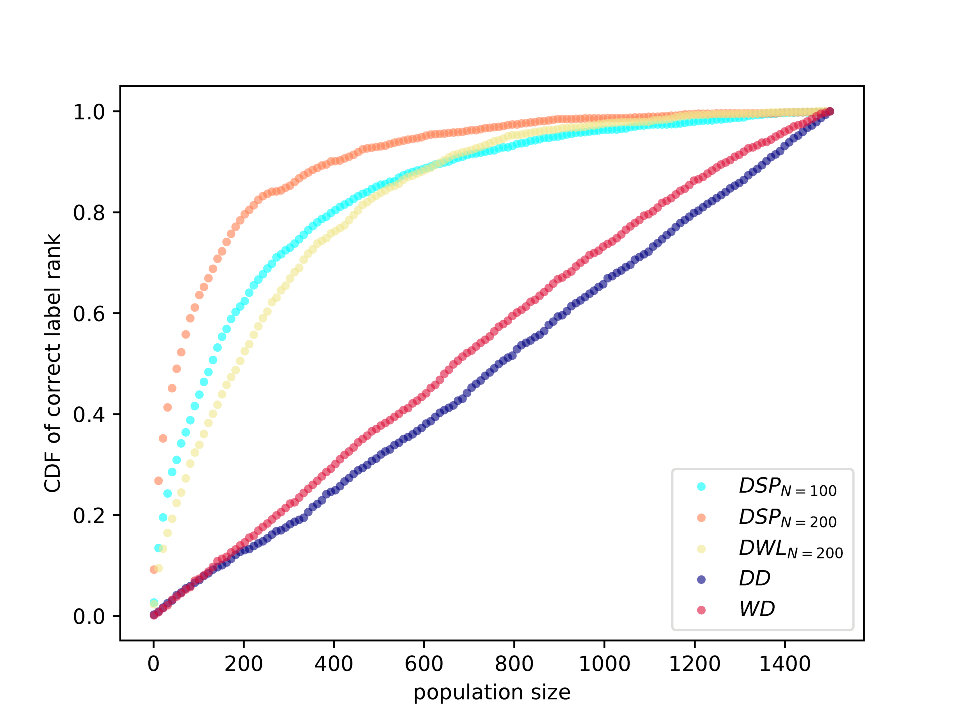
\includegraphics[width=0.8\linewidth]{\MyPath/fig/kernels_evaluation.pdf}
	\caption{\emph{CDF} of true rank over the population according to different kernels.}
	\label{fig:kernels_evaluation}
\end{figure}

The best overall performance is achieved by the \emph{DSP} kernel on graphs pruned to $ 200 $ nodes.
In particular, this kernel places the true identity among the closest 10 networks for $10\%$ of the individuals, and among the closest $ 200 $ networks for $ 80\%$ of the population.
The Shortest-Path kernel has an intuitive interpretation in the case of mobility networks, since its atomic substructures take into account the hop distances among the locations in a user's mobility network and the popularity categories of the departing and arrival location.
The deep variant can also account for variation at the level of such substructures, which are more realistic when considering the stochasticity in the mobility patterns inherent to our dataset.

The best performance of the Weisfeiler-Lehman kernel is achieved by its deep variant for $ h=2 $ iterations of the \emph{WL} test for a mobility network pruned to $200$ nodes.
This phenomenon is explainable via the statistical properties of the mobility networks.
As we saw in~\cref{sec:data-stats}, the networks display power law degree distribution and small diameters.
Taking into account the steps of the \emph{WL} test, it is clear that these topological properties will lead the node relabeling scheme to cover the entire network after a very small number of iterations.
Thus local structural patterns will be described by few features produced in the first iterations of the test.
Furthermore, the feature space of the kernel increases very quickly as a function of $ h $, which leads to sparsity and low levels of similarity over the population of networks.

Histograms of length $10^3$ were also computed for the unweighted and weighted degree distributions and passed through a Gaussian RBF kernel.
We can see that the degree distribution gives almost a random ranking, as it is heavily dependent on the network size.
When including the normalized edge weights, the \emph{WD} kernel only barely outperforms a rand\label{key}om ranking.
Repetitions on pruned versions did not improve the performance and are not presented for brevity.

Based on the insights obtained from our experiment, we can make the following observations with respect to attributes of individual mobility and their impact on the identifiability of networks:
%

\begin{figure*}[]
	\centering
	\begin{minipage}[b]{.45\textwidth}
		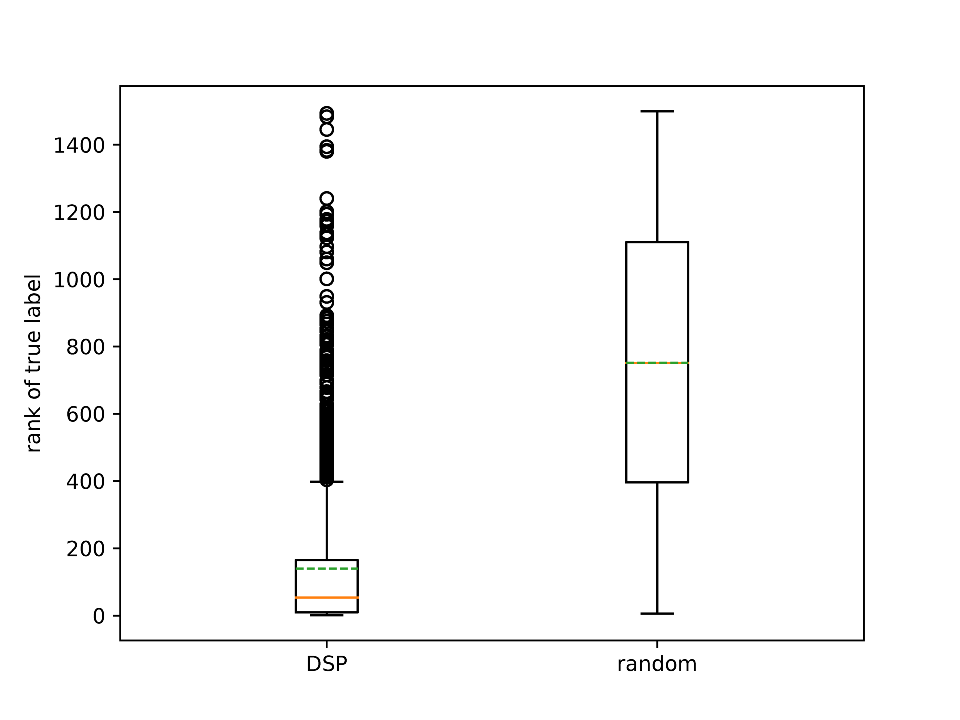
\includegraphics[width=1.2\linewidth]{\MyPath/fig/rank_correct_.pdf}
		\caption{{Boxplot of rank for the true labels of the population according to a Deep Shortest-Path kernel and to a random ordering.}}
		\label{fig:rank_correct}
	\end{minipage}\qquad
	\begin{minipage}[b]{.45\textwidth}
		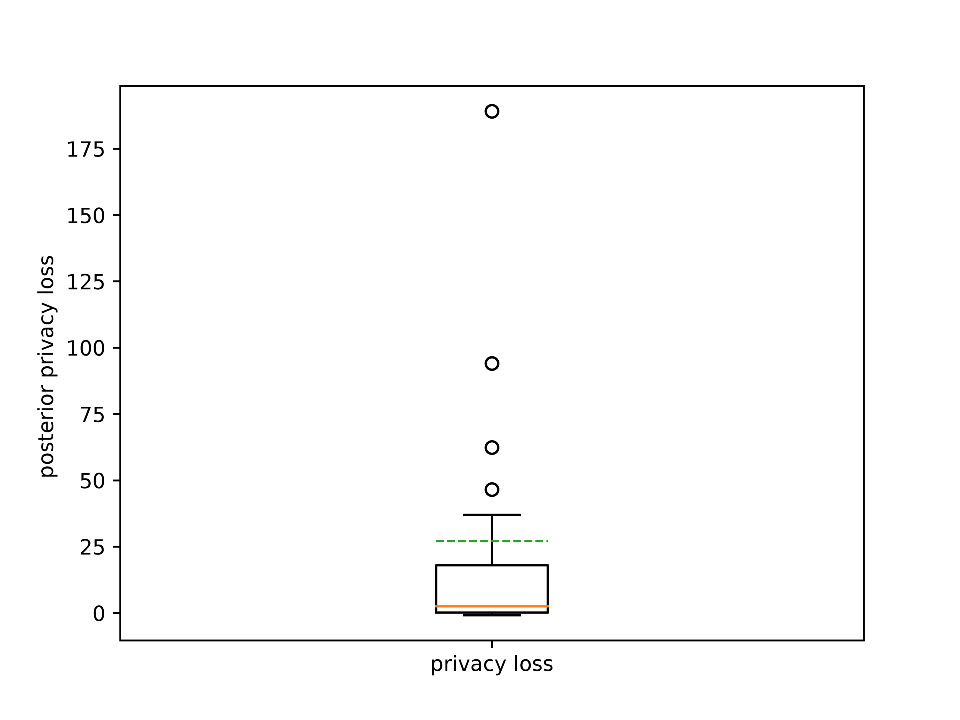
\includegraphics[width=1.2\linewidth]{\MyPath/fig/posterior_privloss_.pdf}
		\centering \caption{{Privacy loss over the test data of our population for an adversary adopting the informed policy of~\eqref{eq:inverse_rank}. Median privacy loss is 2.52.}}
		\label{fig:privloss}
	\end{minipage}
\end{figure*}


\begin{itemize}
	\item \textbf{Location pruning}: Reducing the number of nodes (locations) in a mobility network does not necessarily make it more privacy-preserving.
	On the contrary, if location pruning is done by keeping the most frequently visited locations, it can enhance reidentification.
	In our experiments we obtain similar, or even enhanced, performance for graph kernels when applying them on increasingly pruned networks with size down to $100$ locations.

	\item \textbf{Transition pruning}: Including very rare transitions in longitudinal mobility does not add discriminative information.
	We consistently obtained better results when truncating the long tail of edge weight distribution, which led us to analyze versions of the networks where $40\%$ of the weakest edges were removed.
	\item \textbf{Frequency information of locations}: The frequency of visits to nodes in the mobility network allows better ranking by kernels which support node attributes, e.g.\ Weisfeiler-Lehman and Shortest-Path kernel.
	This information should follow a coarse scheme, in order to compensate for the temporal variation of location popularity in mobility networks.
	\item \textbf{Directionality of transitions}: Directionality generally enhances the identifiability of networks and guides the similarity computation when using Shortest-Path kernels.
\end{itemize}



\subsection{Quantification of Privay Loss}



The Deep Shortest-Path kernel on top$-200$ networks offers the best ranking of identities for the test networks.
As observed in~\cref{fig:rank_correct}, the mean of the true rank has been shifted from $ 750 $ to $ 140 $ for our population.
In addition, the variance is much smaller: approximately $ 218 $, instead of $ 423 $ for the random ordering.

The obtained ordering implies a significant decrease in user privacy, since the ranking can be leveraged by an adversary to determine the most likely matches between a training mobility network and a test mobility network.
The adversary can estimate the true identity of a given test network $ G' $, as suggested in~\cref{sec:threat-model}, applying some simple probabilistic policy that uses pairwise similarity information. For example, let us examine the privacy loss implied by update rule in~\eqref{eq:adversarial_rule} for  \mbox{function $ f$}:

\[
f\left(K_{\text{DSP}}(G_i, G')\right) =\frac{1}{\text{rank}\left(K_{DSP}(G_i, G')\right)}.
\label{eq:inverse_rank}
\]

This means that the adversary updates her probability estimate for the identity corresponding to a test network, by assigning to each possible identity a probability that is inversely proportional to the rank of the similarity between the test network and the training network corresponding to the identity.

From equation~\eqref{eq:privloss}, we can compute the induced privacy loss for each test network, and the statistics of privacy loss over the networks of the Device Analyzer population.
\cref{fig:privloss} demonstrates considerable privacy loss with a median of $ 2.52 $.
This means that the informed adversary can achieve a median deanonymization probability $3.52$ times higher than an uninformed adversary.
Moreover, the positive mean of privacy loss ($ {\approx  27}$) means that the probabilities of  the true identities of the test networks have, on average, much higher values in the adversarial estimate compared to the uninformed random strategy.
Hence, revealing the kernel values makes an adversarial attack easier.

\subsection{Defense Mechanisms }

The demonstrated privacy leakage motivates the quest
for defense mechanisms against this category of attacks.
There are a variety of techniques which we could apply in order to \emph{reduce the recurring patterns of an individual's mobility network over time} and \emph{decrease the diversity of mobility networks across a population}, and therefore enhance the privacy inherent in these graphs.
Examples include noise injection on network structure via several strategies: randomization of node attributes, perturbations of network edges, or node removal.
It is currently unclear how effective such techniques will be, and what trade-off can be achieved between utility in mobility networks and the privacy guarantees offered to individuals whose data the graphs represent.
Moreover, it seems appropriate to devise kernel-agnostic techniques, suitable for generic defense mechanisms.
For example, it is of interest to assess the resistance of our best similarity metric to noise, as the main purpose of deep graph kernels is to be robust to small dissimilarities at the substructure level.

We think this study is important for one further reason: kernel-based methods allow us to apply a rich toolbox
of learning algorithms without accessing the original datapoints, or their feature vectors, but instead by using their kernel matrix.
Thus studying the anonymity associated with kernels is valuable for ensuring that such learning systems do not leak privacy of the original data.
We leave this direction to future work.
